\section*{Step 5}

\begin{custombox}[label={box:Q5}]{Step 5}
	Review \textbf{\texttt{Sklearn}} documentation to understand and experiment with a few more ($2$ - $3$) regression methods, in addition to the ones listed above, and document the outcomes of your experiments.
\end{custombox}

\subsubsection*{Ridge Regression (Ridge)}

\begin{itemize}
    \item \textbf{Overview:} Ridge Regression is a linear regression model that includes L2 regularization. It is used to prevent overfitting by penalizing large coefficients in the regression model.
    \item \textbf{Key Parameters:}
    \begin{itemize}
        \item \texttt{alpha}: Regularization strength. Must be a positive float. Larger values specify stronger regularization.
        \item \texttt{copy\_X}: Boolean value indicating whether to copy the input data. Default is \texttt{True}.
        \item \texttt{max\_iter}: Maximum number of iterations for the optimization algorithm. Default is \texttt{None}.
        \item \texttt{tol}: Tolerance for the optimization. Default is \texttt{1e-3}.
        \item \texttt{solver}: Algorithm used to compute the solution. Options include \texttt{auto}, \texttt{svd} (singular value decomposition), \texttt{cholesky} (direct method), \texttt{lsqr} (least squares with regularization), and \texttt{sparse\_cg} (conjugate gradient for sparse matrices).
        \item \texttt{fit\_intercept}: Boolean value that indicates whether to calculate the intercept. Default is \texttt{True}.
        \item \texttt{normalize}: Boolean value for whether to normalize the features before regression. Default is \texttt{False}.
    \end{itemize}
\end{itemize}

\begin{figure}[H]
	\centering
	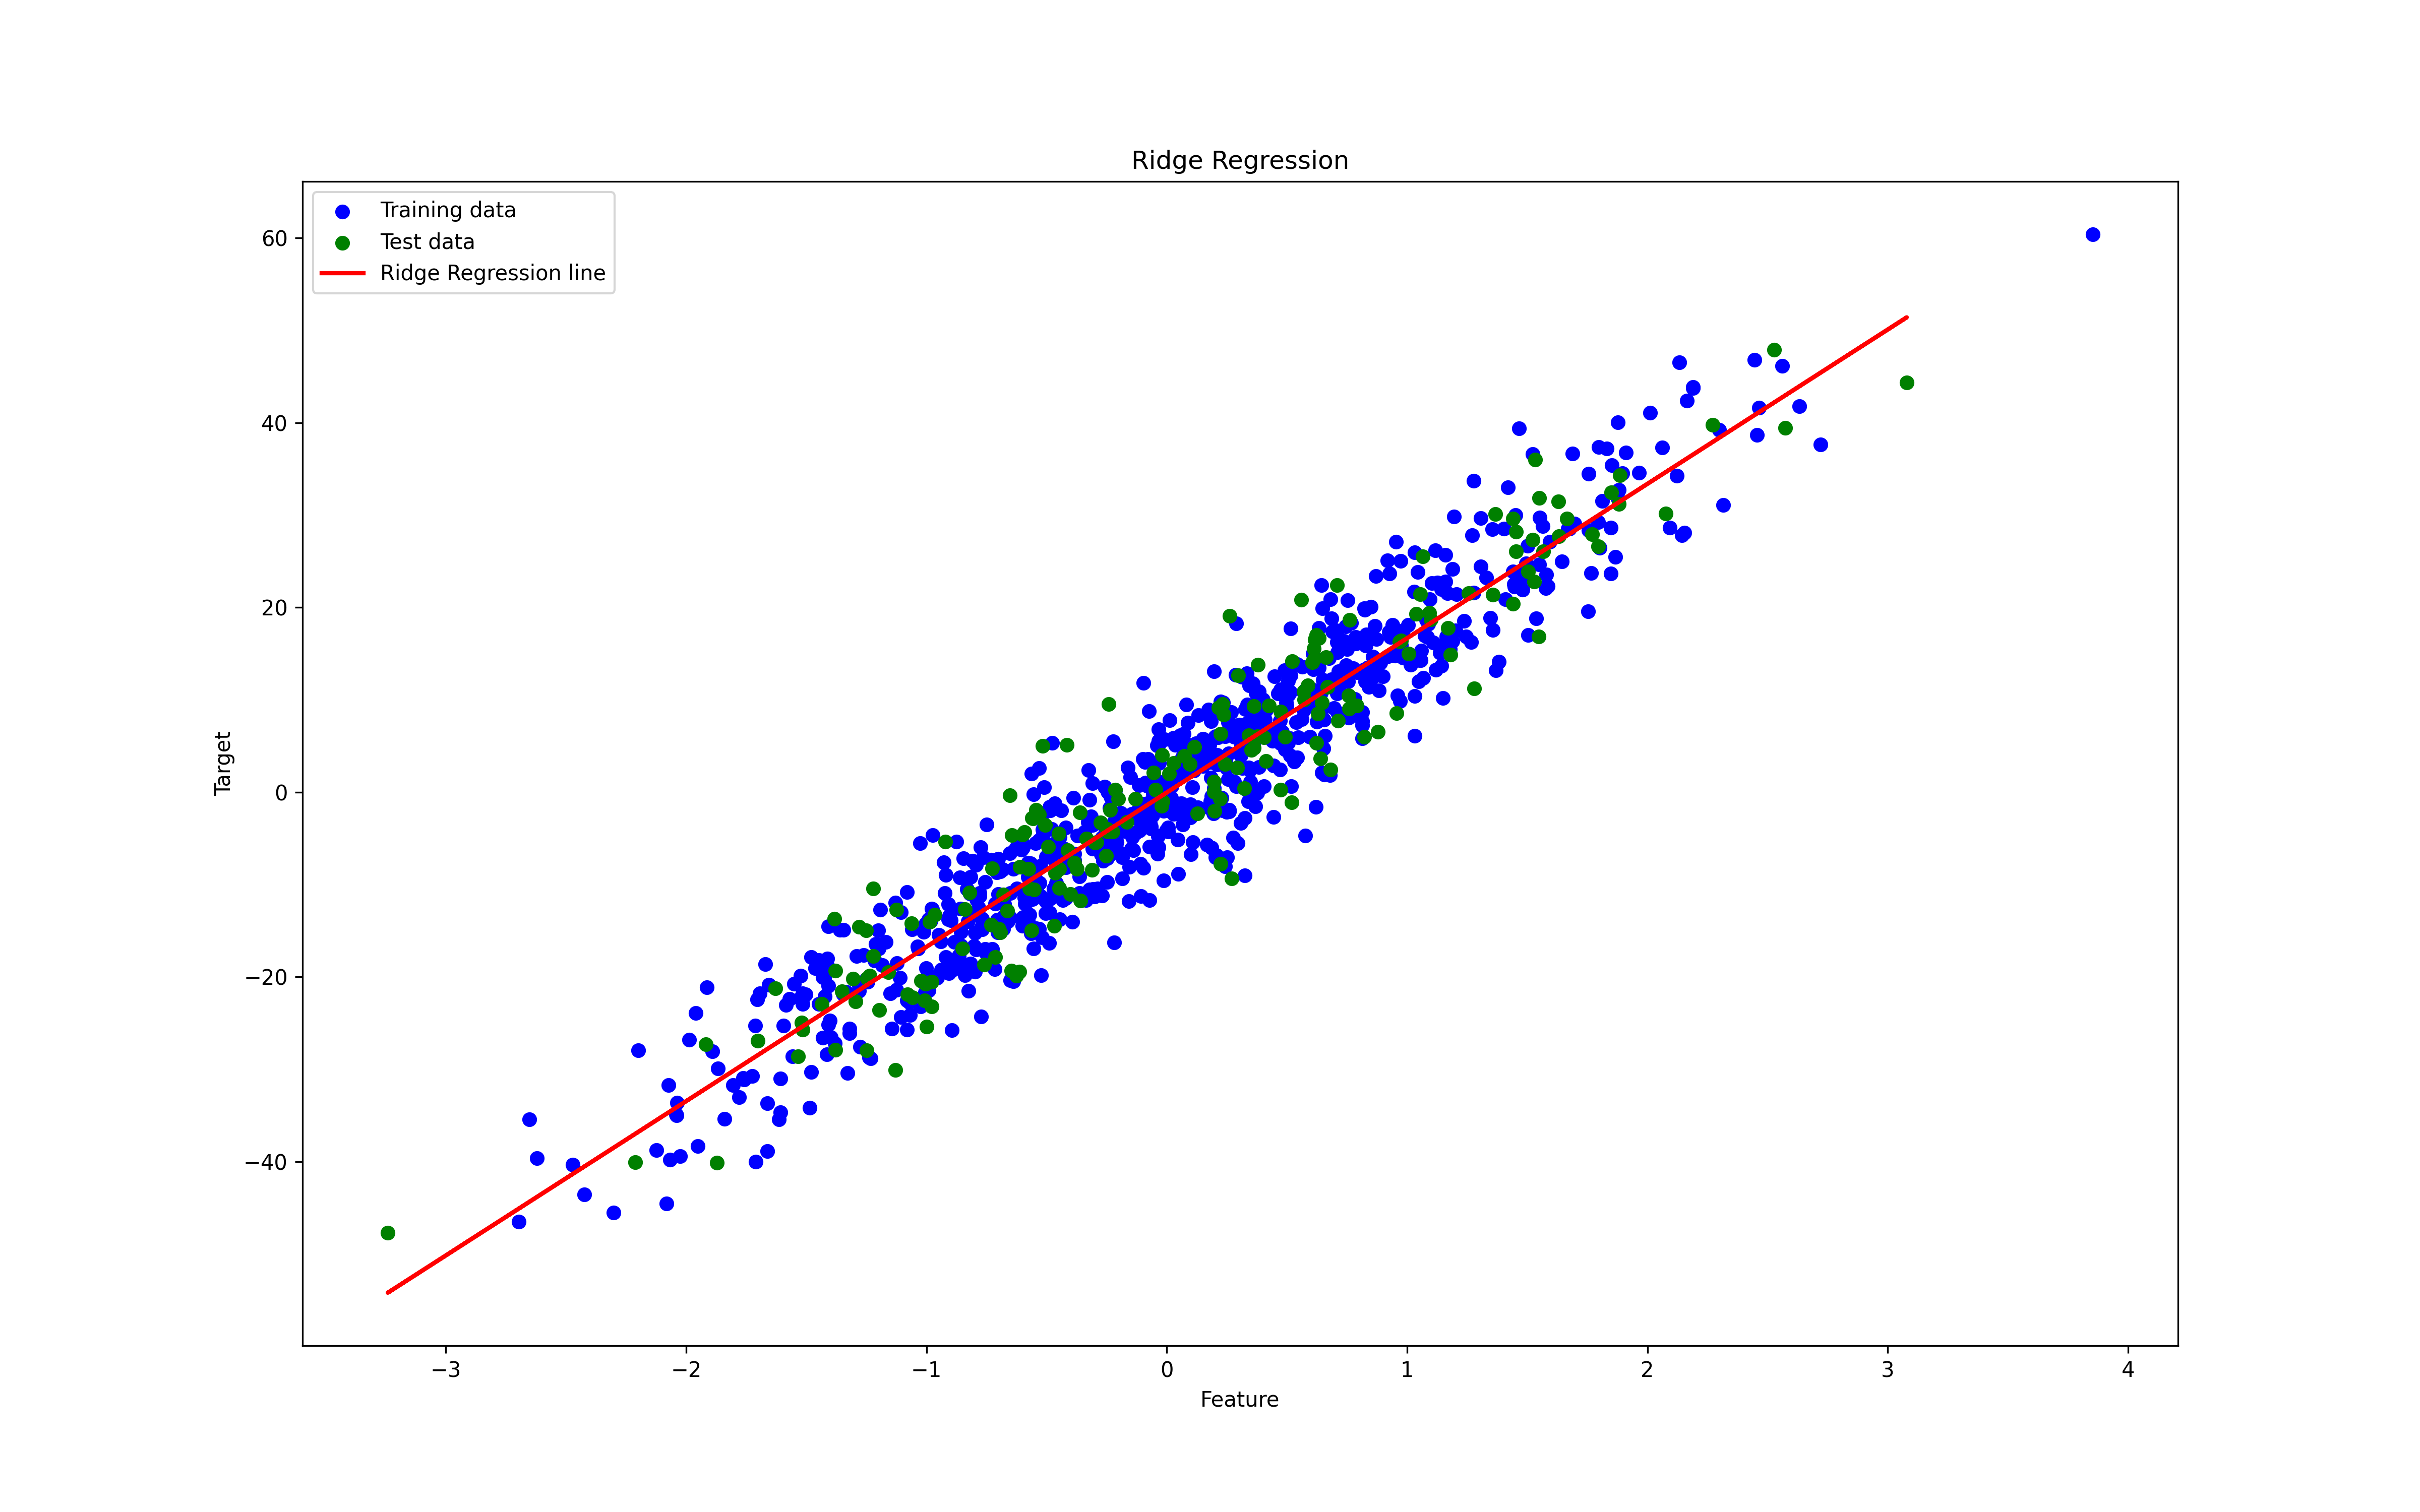
\includegraphics[width=0.95\textwidth]{./Images/Ridge-Regression.png}
	\caption{Ridge Regression}
	\label{fig:ridge-regression}
\end{figure}

\begin{lstlisting}[language=Python, caption=Ridge Regression Example]
from sklearn.linear_model import Ridge
from sklearn.datasets import make_regression
from sklearn.model_selection import train_test_split

X, y = make_regression(n_samples=1000, n_features=1, noise=5, random_state=42)
X_train, X_test, y_train, y_test = train_test_split(X, y, test_size=0.2, random_state=42)

ridge_model = Ridge(alpha=1.0)
ridge_model.fit(X_train, y_train)
y_pred = ridge_model.predict(X_test)
\end{lstlisting}

\subsubsection*{Lasso Regression (Lasso)}

\begin{itemize}
    \item \textbf{Overview:} Lasso Regression is a linear regression model that includes L1 regularization. It not only prevents overfitting but also performs feature selection by shrinking some coefficients to zero.
    \item \textbf{Key Parameters:}
    \begin{itemize}
        \item \texttt{alpha}: Regularization strength. Must be a positive float. Larger values increase regularization, which can set more coefficients to zero.
        \item \texttt{max\_iter}: Maximum number of iterations for the optimization algorithm. Default is \texttt{1000}.
        \item \texttt{tol}: Tolerance for the optimization. Default is \texttt{1e-4}. Smaller values require higher precision.
        \item \texttt{fit\_intercept}: Boolean value indicating whether to calculate the intercept. Default is \texttt{True}.
        \item \texttt{normalize}: Boolean value to normalize the features before regression. Default is \texttt{False}.
        \item \texttt{selection}: Strategy for selecting features. Options are \texttt{cyclic} (default) or \texttt{random}.
    \end{itemize}
\end{itemize}

\begin{figure}[H]
	\centering
	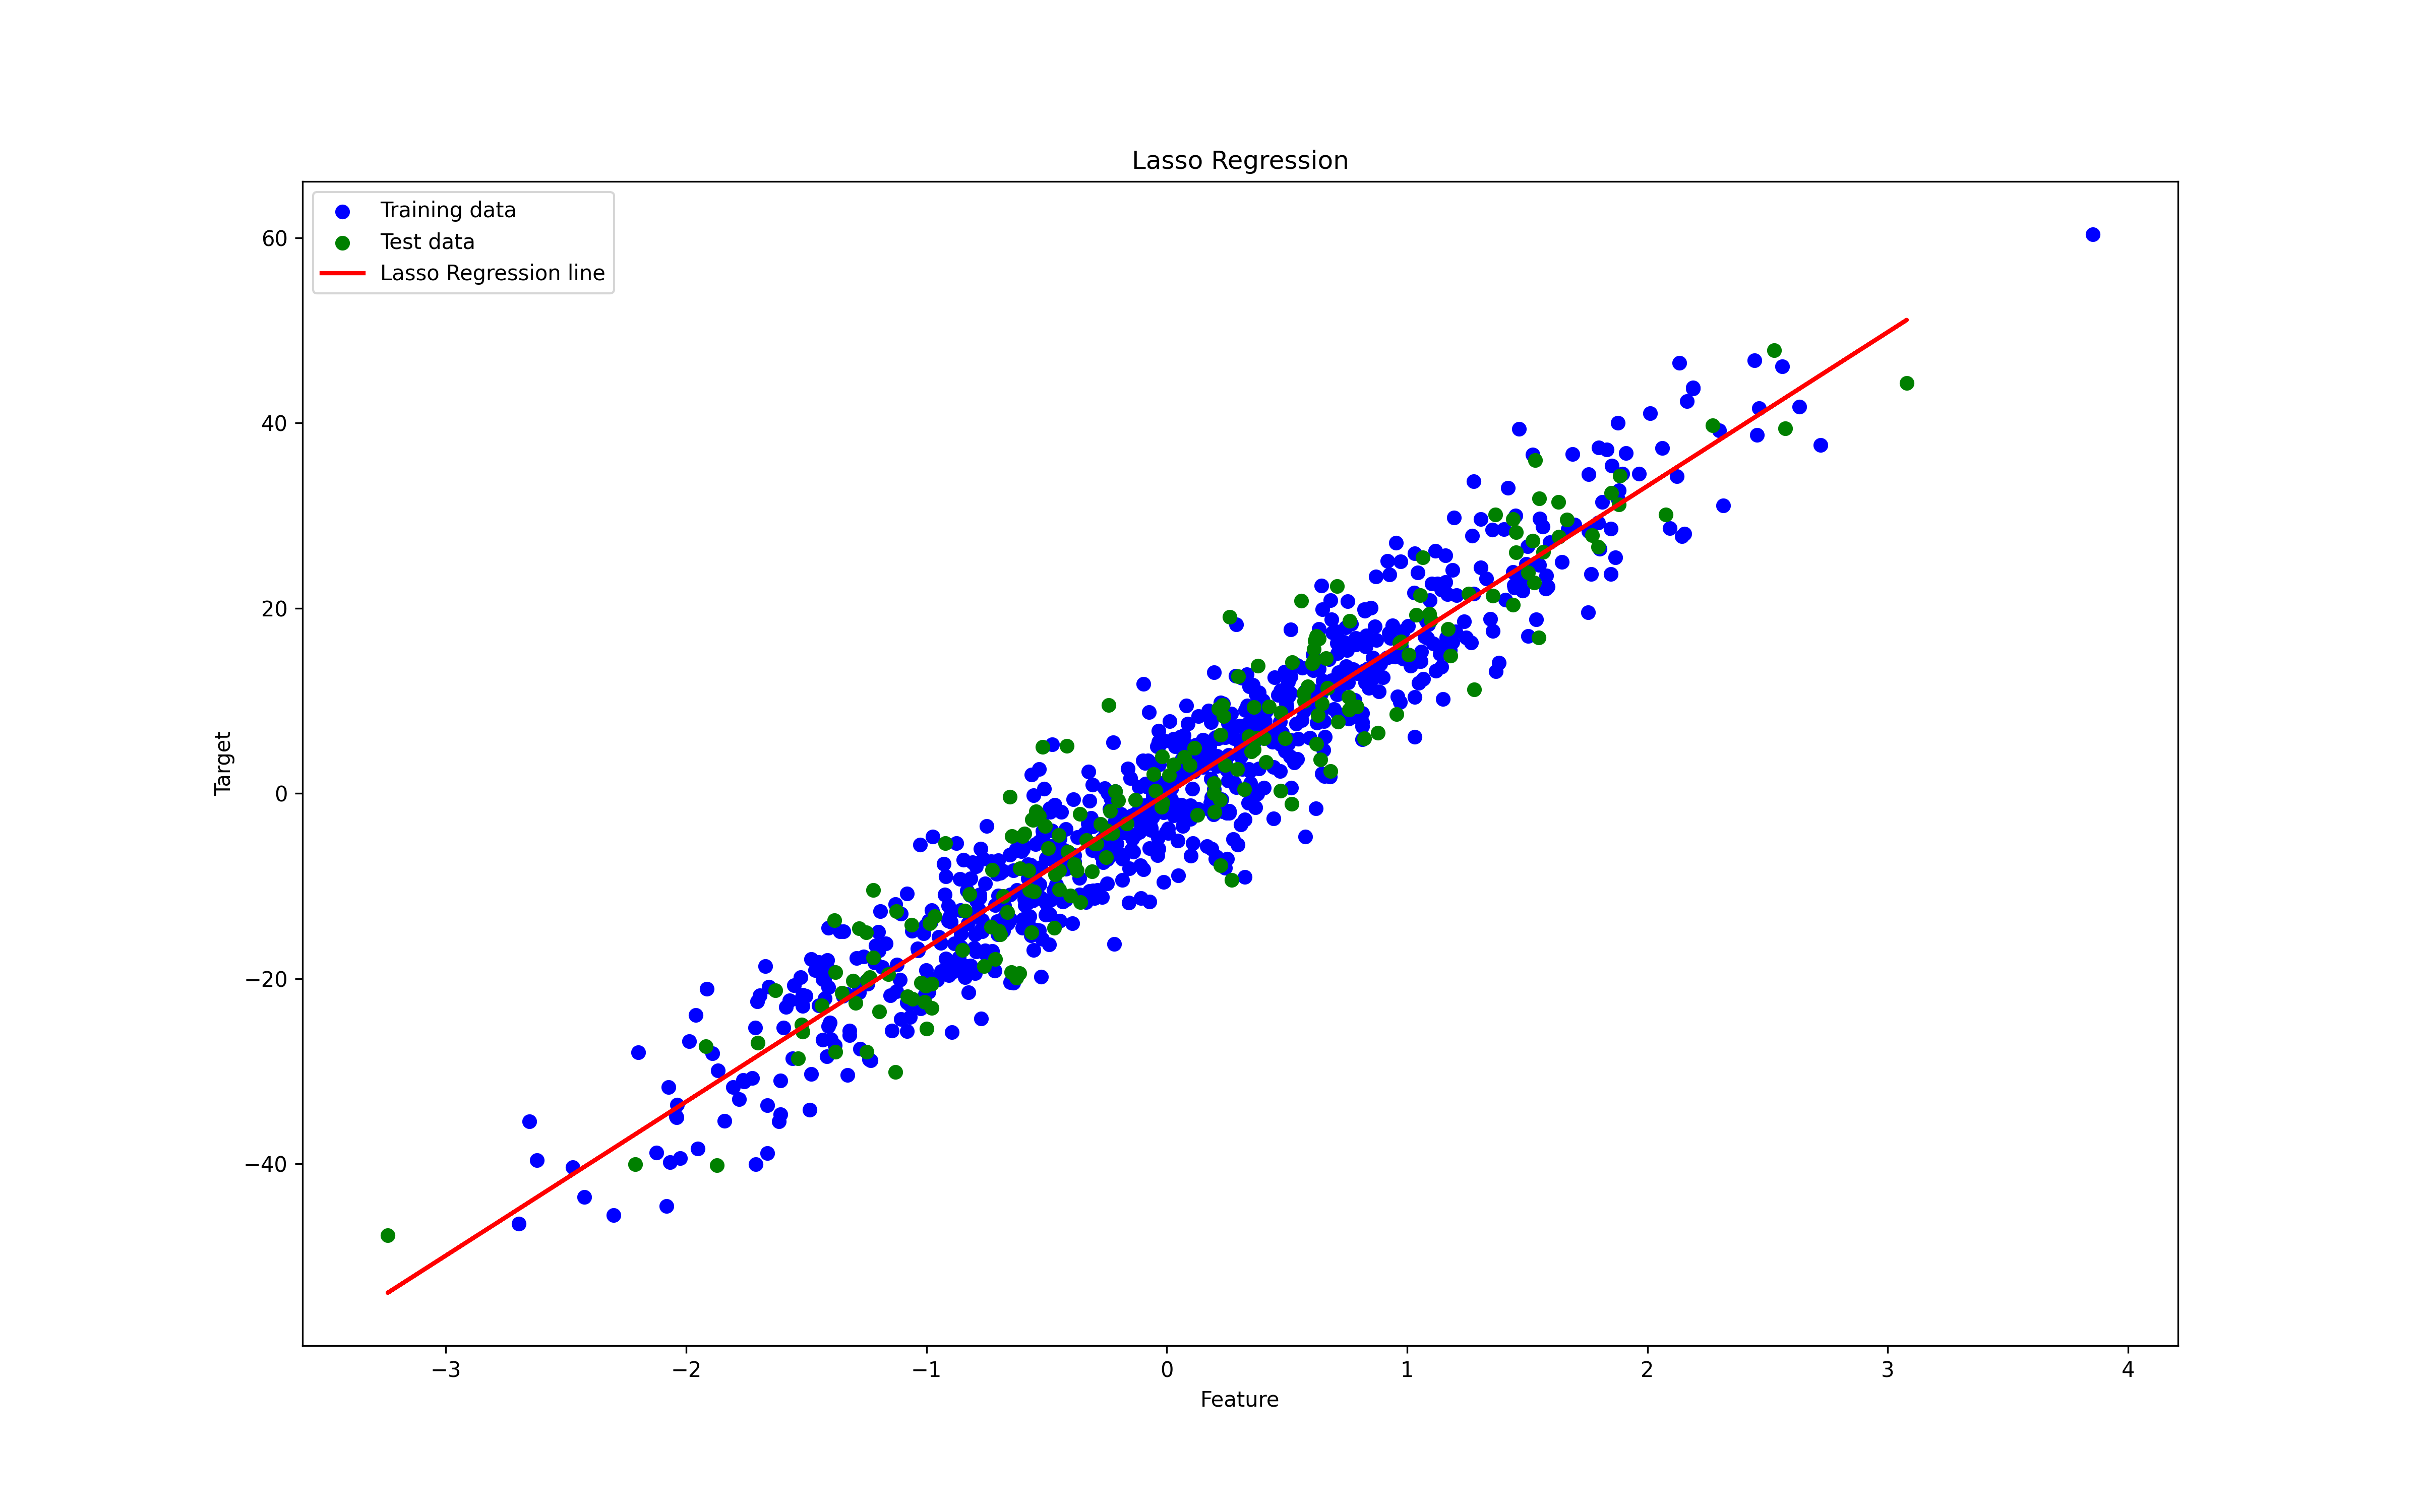
\includegraphics[width=0.95\textwidth]{./Images/Lasso-Regression.png}
	\caption{Lasso Regression}
	\label{fig:lasso-regression}
\end{figure}

\begin{lstlisting}[language=Python, caption=Lasso Regression Example]
from sklearn.linear_model import Lasso
from sklearn.datasets import make_regression
from sklearn.model_selection import train_test_split

X, y = make_regression(n_samples=1000, n_features=1, noise=5, random_state=42)
X_train, X_test, y_train, y_test = train_test_split(X, y, test_size=0.2, random_state=42)

lasso_model = Lasso(alpha=0.1)
lasso_model.fit(X_train, y_train)
y_pred = lasso_model.predict(X_test)
\end{lstlisting}


\subsubsection*{Gradient Boosting Regressor}

\begin{itemize}
    \item \textbf{Overview:} Gradient Boosting Regressor is an ensemble learning technique that builds models sequentially. Each model corrects the errors of the previous one, combining their predictions to improve performance.
    \item \textbf{Key Parameters:}
    \begin{itemize}
        \item \texttt{n\_estimators}: Number of boosting stages to be run. Default is \texttt{100}. More estimators generally improve performance but also increase training time.
        \item \texttt{learning\_rate}: Step size for each boosting stage. Default is \texttt{0.1}. Lower values improve model generalization but require more stages.
        \item \texttt{max\_depth}: Maximum depth of individual trees. Default is \texttt{3}. Deeper trees capture more complex patterns but may overfit.
        \item \texttt{min\_samples\_split}: Minimum number of samples required to split an internal node. Default is \texttt{2}.
        \item \texttt{min\_samples\_leaf}: Minimum number of samples required to be at a leaf node. Default is \texttt{1}.
        \item \texttt{subsample}: Fraction of samples used to fit each base learner. Default is \texttt{1.0}. Values less than 1.0 can help with regularization.
    \end{itemize}
\end{itemize}

\begin{figure}[H]
	\centering
	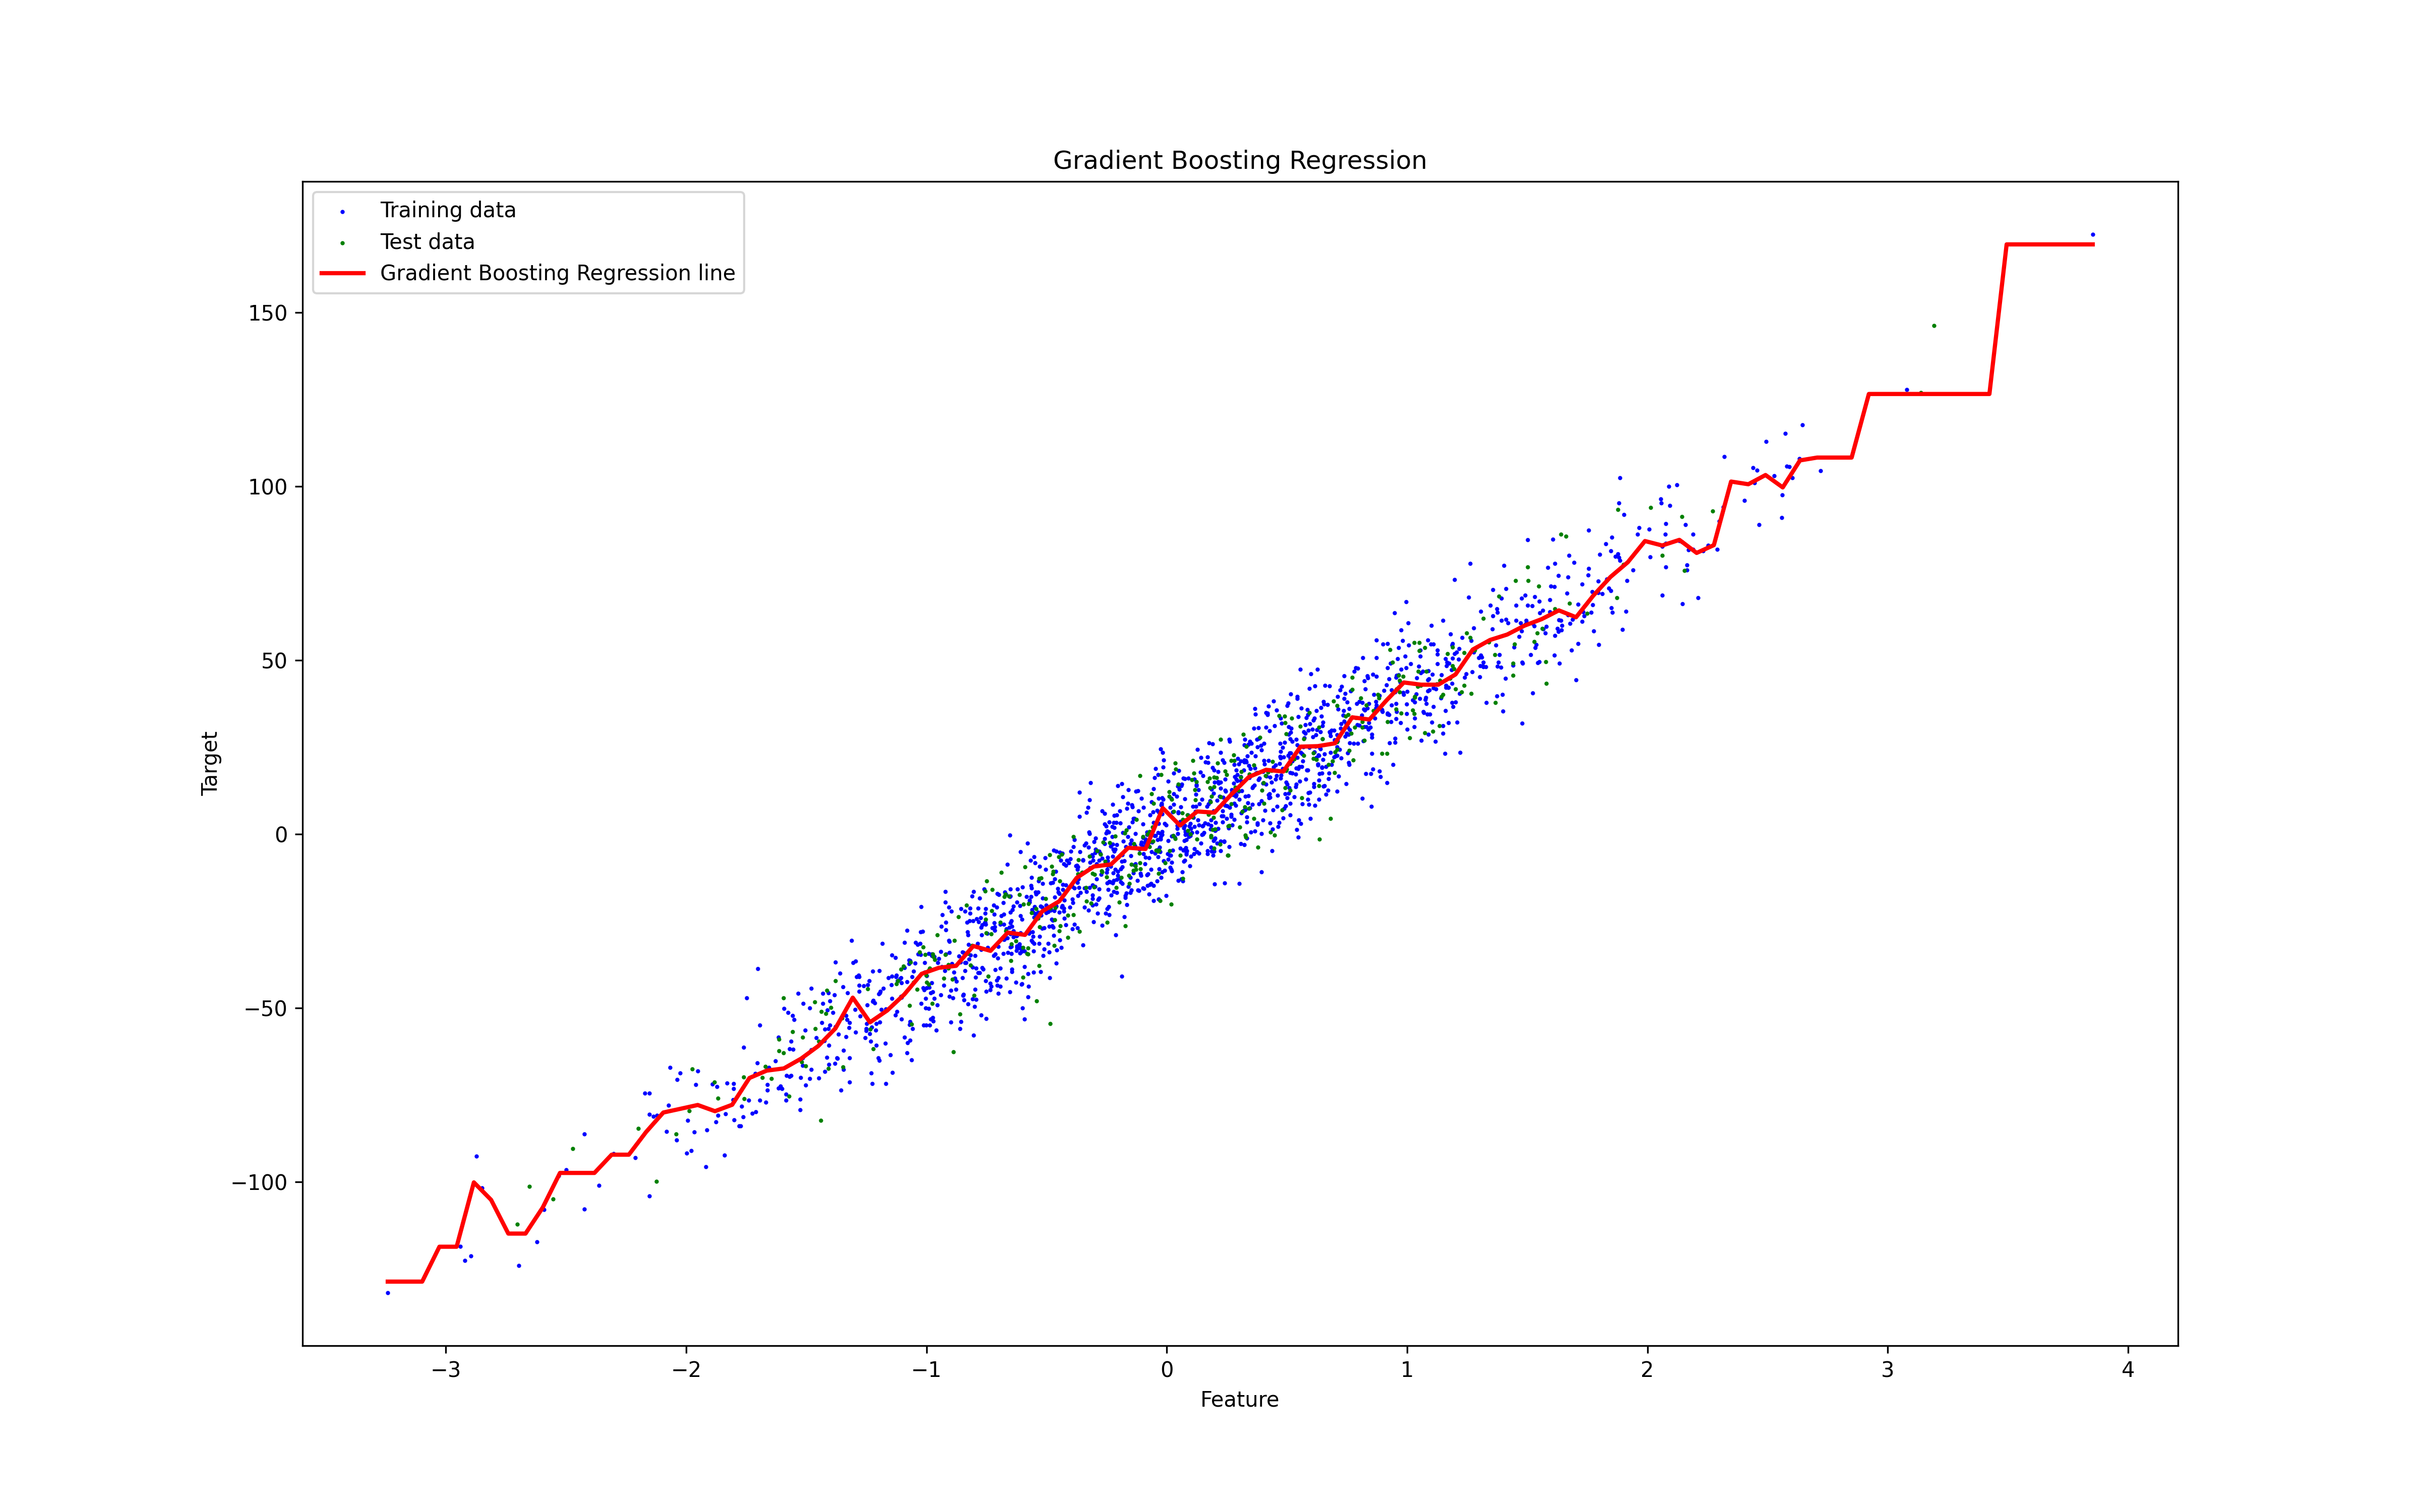
\includegraphics[width=0.85\textwidth]{./Images/Gradient-Boosting-Regression.png}
	\caption{Gradient Boosting Regressor}
	\label{fig:gradient-boosting-regressor}
\end{figure}

\begin{lstlisting}[language=Python, caption=Gradient Boosting Regressor Example]
from sklearn.ensemble import GradientBoostingRegressor
from sklearn.datasets import make_regression
from sklearn.model_selection import train_test_split

X, y = make_regression(n_samples=2000, n_features=1, noise=10, random_state=42)
X_train, X_test, y_train, y_test = train_test_split(X, y, test_size=0.2, random_state=42)

gbr_model = GradientBoostingRegressor(n_estimators=100, learning_rate=0.1, max_depth=3, random_state=42)
gbr_model.fit(X_train, y_train)
y_pred = gbr_model.predict(X_test)
\end{lstlisting}
